\chapter{Data Quality}
\label{Sec:DataQuality}
Various projects today is focused on gathering data and analysing it. The gathered data is used for obtaining behaviours, habits and properties of the observed objects. This is done by using powerful statistical leaning algorithms, that are able to deduce these properties from the data. This approach is called data driven development, since the success is mainly determined by the data and not the algorithm. 

When data is the central role of the system, the quality of the data are very important. Poor data can lead to wrong assumptions, and have a negative effect on the application. Choosing the correct dataset is therefore a key factor \cite{RefWorks:3}. Looking at the quality of the data can help you chose what dataset to use. Data quality can be described many ways, one of the more formal is from the ISO 8402 standard that describes quality as: 

\begin{adjustwidth}{2.5em}{2.5em}
\emph{"The totality of characteristics of an entity that bear upon its ability of satisfy stated and implied needs"} \cite{RefWorks:5}.
\end{adjustwidth}

This indicate that data quality is something that is very depended on the intended application, and is therefore hard to generalize. 

Quality of data is a subject that is gaining more and more attention due to the fact that the quantity of data available is larger than ever before. This forces researchers to choose between datasets, and a notion of quality in the dataset can help them choose. The heavy growth in available data is a result of projects that are moving data gathering from controlled labs, to the public. Many of these projects is citizen science projects, where it is the citizens who collect the data, and not the researchers \cite{RefWorks:2}. This enables researchers to gather enormous amount of data, but they are no longer in control of the conditions the data is collected in, which introduces errors and other quality decreasing factors. 

Non intrusive load monitoring is a topic that have been in focus in the past years. This is due to the rise of the smart meters, that makes it possible to measure at faster intervals, and collect the data on online services form real environments. But the smart meters architecture is designed after billing and regulation purposes, and not load monitoring. The network architecture is therefore often based on the unreliable \ab{UDP}[user datagram protocol], since it is more important to get the current information fast, than get all information. This courses a lot of packets to be lost in transition, which can degrade the completeness quality of the signal. The missing data can be a problem for load monitoring, since many methods of load disaggregation is based on learning techniques. The quality of the signal can also help identify if the collected data is suitable as a training set. 


\section{Quality Criteria}
It is not uncommon that different areas of research has its own quality criteria. This is due to the fact that quality is a very domain specific subject. One of the areas that have been dealing with citizen data for many years is the Geographic information area, that are used for maps, weather prediction and climate research. They have come up with several ways of describing quality in spatial data \cite{RefWorks:7}. Method for defining quality in time series data have also been developed  \cite{RefWorks:6}. To better define quality criteria in the smart meter data inspiration from related work is used.

\subsection{Related Work}
Data quality is an area that recently have become a hot topic, due to the wast quantity of data. Many researchers strive to make tools that better can analyse data quality in different areas. In the area of spatial data is a \emph{"Quality and Workflow tool"} being developed by the University of Wageningen \citep{RefWorks:8}. The objective is to help researchers select the best suited data for a given data driven project. It does this by looking at different quality criteria, given by the user or found in standards for spatial data. 

In bioinformatics is a tool named QCScreen developed to help create better dataset to metabolomics studies. In metabolomics studies is dataset often created by joining information from several different experiments of various quality. By using tools that can check the data quality and consistency to determine if a dataset is suitable for further processing, they are able to greatly improve the test results \citep{RefWorks:9}.
 
In the article \emph{Taking a big Data approach to data quality in a citizen science project}\citep{RefWorks:2} they talk about how quality assessment can be used to rate the believe on your data, and how to improve data collected in citizen science. The project focuses on bird observations, done by users on their smartphones. They improve the quality by disallowing the user to send incomplete datasets to the database, and in this way forcing the user to only deliver high quality information. They then cross check the information with information from people in the same area, to see if it varies greatly. 

In the \ab{NILM} research area have data quality also emerge when talking about comparison between dataset. One of the tools working with this is the \ab{NILMTK} project \citep{RefWorks:21}. In this they look at a series of quality parameter that can be used specifically for \ab{NILM}. They point out that looking at the energy consumption observed by the main meter in relation to what is observed at the sub-meters tells a lot about the training set. This is since the success ratio of disaggregating appliances consuming lot of energy is higher than once that only consume a little. 

One of the things all the methods have in common is trying to look at the completeness of the data. Some of the most low level criteria is the sample availability. The sample availability describes how many samples there is collected in relation to the expected collection amount, and look at how the samples are distributed in the measurement period. It is also seen that the activity is a good quality metric since a good data set must contain both areas with activity and areas without. 

\section{Quality In SmartHG Citizen Data}
As a part of the SmartHG project 25 households have been equipped with meters on selected appliances and the main meter. The data collected from this experiment are prone with errors due to malfunctioning test equipment or unexpected interference from the resident which have resulted in offline measurement equipment for periods of time. Examples on unexpected interference could be if the resident is unplugging the measurable equipment, or turning off the power socket that supply's it. Unstable network does further degrade the signal, since the measurement equipment uses a lossy network. 

\subsection{Completeness And Activity}
The SmartHG data is intended for appliance recognition, and the quality must be assessed with this in mind. The completeness and the activity in the data is therefore important. 

\begin{figure}[H]
\centering
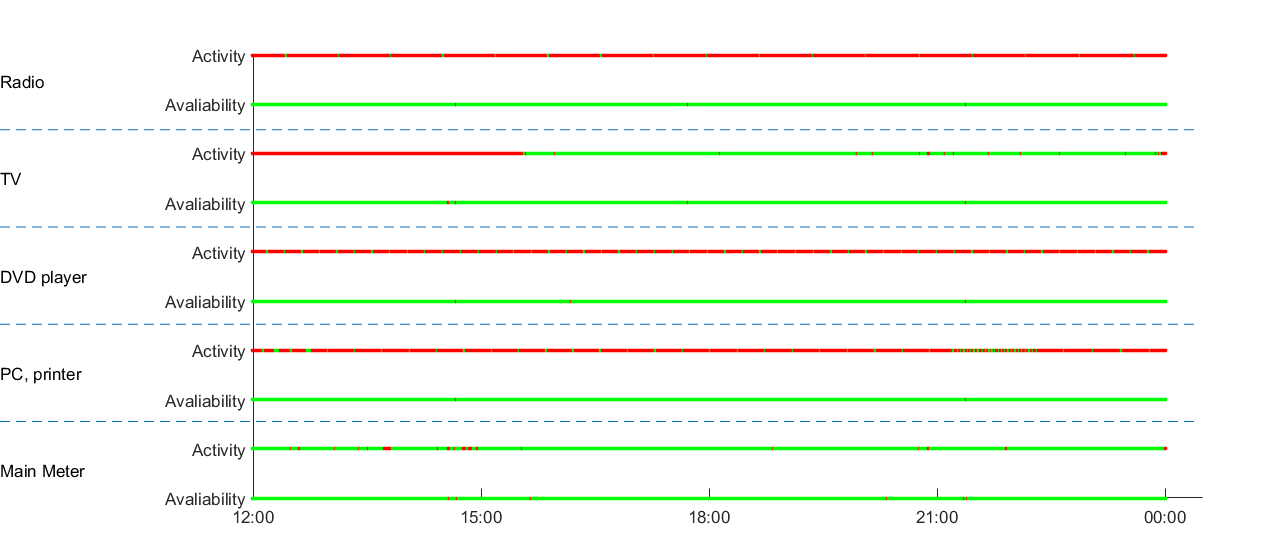
\includegraphics[width=1\textwidth]{billeder/Test.png}
\caption{12 hour overview of house 10}
\label{fig:12HRes}
\end{figure}

On figure \ref{fig:12HRes} is a 12 hour overview of the data in house 10 from the 16/8/2015. Here we see the sample availability and activity of the five different meters in the house. The availability is shown as a line where green is indicating that a sample is received as expected, and red shows a missing sample. On the figure it is shown that there is a few samples missing, which is to be expected due to the lossy network architecture. The Activity is also shown as a line, where green indicates activity and red indicates no activity. Activity is defined as a change in the signal, from prior values. From this we can see that the resident have a lot on activity on the TV from around 16:00 to 00:00, which we can presume means that the television is turned on in this period. 

First the availability quality of the data is assessed. The availability quality for a specific period of time $T_n$ for a specific meter $m$, is defined as the amount of samples observed in that timeslot over the expected sample amount. The resolution period $T_P$ for each time period in $T$ is chosen to be one hour. 

\begin{figure}[H]
\begin{picture}(0,140)
\put(0,0){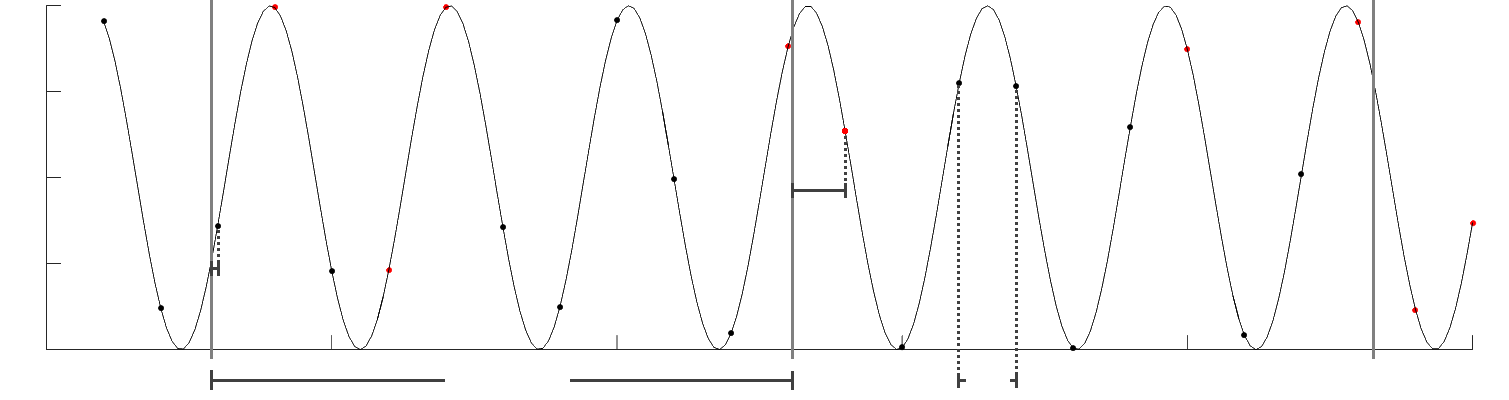
\includegraphics[width=1\textwidth]{billeder/IllustrationQua.png}}
\put(146,0){$T_P$}
\put(65,30){$\phi_{start}^{(m,T_n)}$}
\put(241,47){$\phi_{start}^{(m,T_{n+1})}$}

\put(294,0){$T_s$}

\put(145,130){$T_n$}
\put(325,130){$T_{n+1}$}

\end{picture}
\caption{Illustration of availability analysis}
\label{Fig:IOAA}
\end{figure}

To calculate the amount of samples expected to be in a specific period of time $N_{max}^{(m,T_n)}$ does the sample phase $\phi_{start}^{(m,T_n)}$ for the given period need to be known. On figure \ref{Fig:IOAA} a illustration of a signal, the black dots are the samples and the red dots are the ones that are missing. The sample phase is the time from the beginning of the period $T_n$ and to the first expected sample. This is needed since for a timeslot $T_n$ of a length of $T_P$ the maximum expected sample amount can vary with 1. This is shown in figure \ref{Fig:IOAA} where the period $T_n$ has a potential of having 11 samples, where as period $T_{n+1}$ only can have 10. 

\begin{gather}
		N_{max}^{(m,T_n)} = \floor{ \frac{(T_{P}-\phi_{start}^{(m,T_n)})}{T_s^{(m)}}} + 1 \label{EQ:NMAX} \\
		q^{(m,T_n)} = \frac{N_{observed}^{(m,T_n)}}{ N_{max}^{(m,T_n)} } \label{EQ:QMT}
\end{gather}

As shown on equation \ref{EQ:NMAX} is the maximum number of samples for a meter $m$ in the period $T_n$ calculated by taking the period time $T_P$, corrected with the sample phase $\phi_{start}^{(m,T_n)}$ for the given period, and dividing it with the sample time $T_s$. The quality of the meter is calculated as the ratio of observed samples in the timeslot $T_n$ to the maximum samples, shown in equation \ref{EQ:QMT}. 

To find the quality of a house in a given period $T_n$, that have a set of meters $\mathbf{M}$ with a cardinality of $M$, we take the mean value of all the meter quality's, as shown in equitation \ref{EQ:HQT}.  
\begin{equation}
	\mu_{q^{(\mathbf{M},T_n)}} = \frac{1}{M} \sum_{m \in \mathbf{M}} q^{(m,T_n)}
	\label{EQ:HQT}
\end{equation}



A quality vector $Q$ is constructed for each house. The quality vector contains the house quality found with a period $T_P$ on one hour. This have been done from March $T_1$ to October $T_N$. 

\begin{equation}
	Q^{(\mathbf{M})} = \{ \mu_{q^{(M,T)}} | T \in \{T_1, T_2, ... ,T_n,..., T_N  \} \}
	\label{EQ:HQV}
\end{equation}
This is shown in equation \ref{EQ:HQV} where $\mathbf{M}$ is a set of meters in a given house. This can be graphically shown in figure \ref{fig:SmartHGQuality} where all the houses $Q$ vectors is shown. The color is a gradient running from light green for the best quality to red for bad quality.
\begin{figure}[H]
\centering
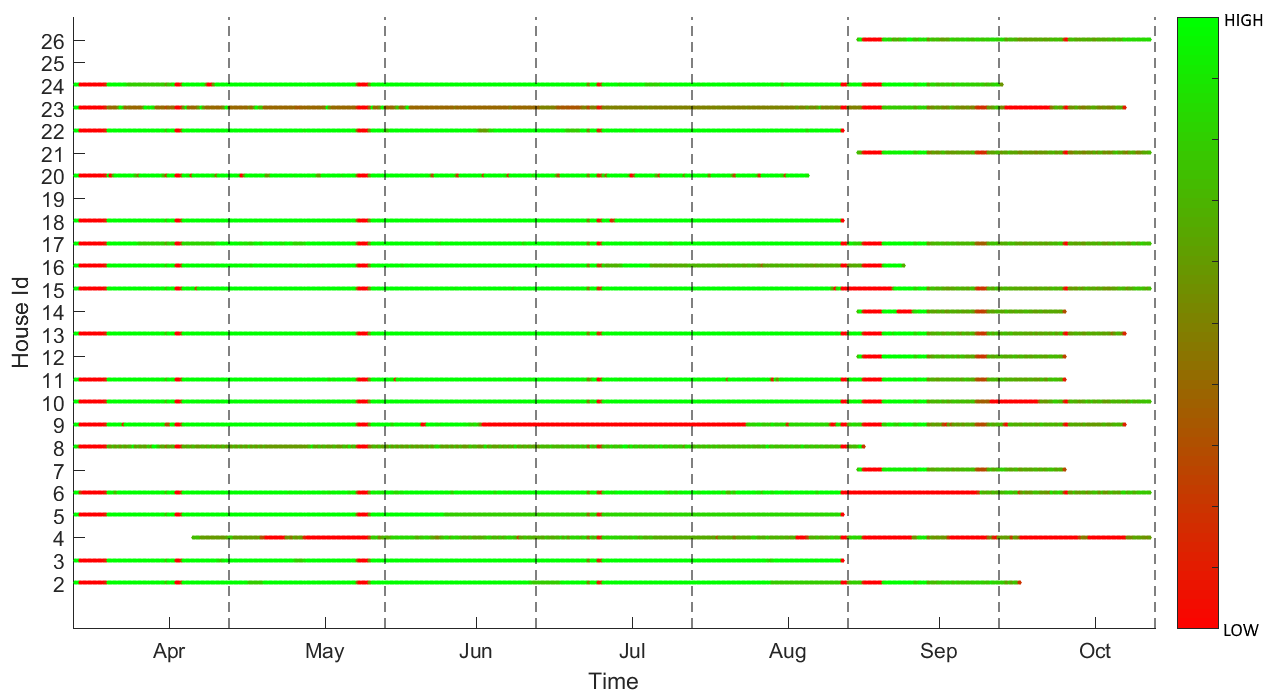
\includegraphics[width=1\textwidth]{billeder/QualityBig.png}
\caption{Quality of houses in SmartHG project}
\label{fig:SmartHGQuality}
\end{figure} 

On figure \ref{fig:SmartHGQuality} is the availability quality shown for the 25 houses in the SmartHG project. When seen on this scale with a analysis resolution on one hour it is hard to see degradation coursed by single sample missing here and there, but meters that have malfunctioned over a longer times shows itself. Since the quality of a house is the mean of several meter quality's, will this most likely appear as darker green spots, since not all meters are malfunctioning at the same time. But there still are some red areas indicating that all the meters in a house is not working. 

There are the red spots that goes through all houses on the exact same time. This indicates that the server receiving the data for all the houses have been down, since it is unlikely that all meters in every house is down at the same time. The conclusion being that red dots most commonly are coursed by the network being unavailable so the client can not sent to the server, or the server is unable to receive. 

It is assumed that the first sample received from a meter happen at the time of meter installation, and the last sample received is the time of meter removal. The meter is assumed to be operating in between these two points in time. On the figure does the coloured $Q$ vector starts at installation time, and ends at removal time. This illustrates how some houses have been operational longer than others. 

Since the data is intended for appliance recognition it is of interest where in the data there is activity, and where there is nothing happening. Both areas are impotent for a \ab{NILM} application in training scenarios. We define activity as area in the data where there is change as described in equation \ref{EQ:CHANGE}.

\begin{equation}
f(x) + \epsilon < f(x+1) \vee f(x) - \epsilon > f(x+1)
\label{EQ:CHANGE}
\end{equation}

Where $\epsilon$ describes a threshold to filter out changes caused by noise. This can also be described as the standard divination over a area is grater than the threshold. The activity is analysed in the available data, and is shown on figure \ref{fig:ActivityMap} where green is high activity and red is non activity. 

\begin{figure}[H]
\centering
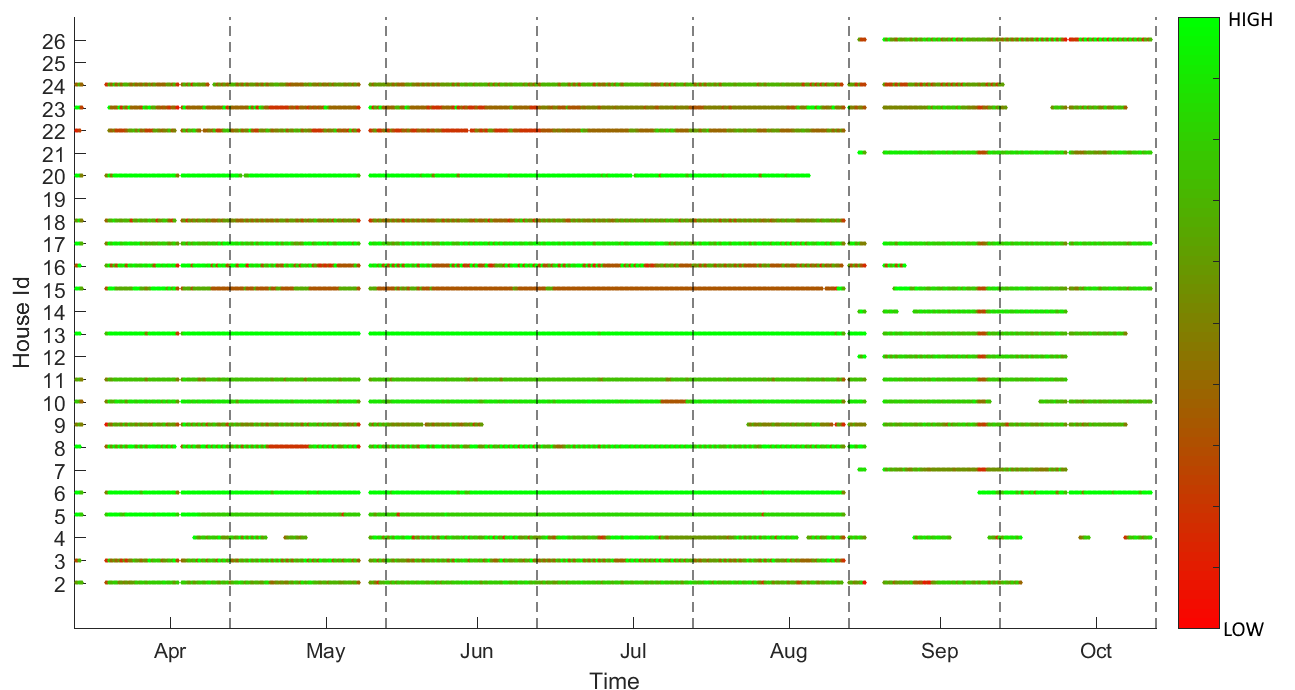
\includegraphics[width=1\textwidth]{billeder/ActivityBig.png}
\caption{Activity of houses in SmartHG project}
\label{fig:ActivityMap}
\end{figure}

The activity shown on figure \ref{fig:ActivityMap} is the average of the activity of the meters in the house. There is almost never a meter that does not have at least a little activity in a house, so a complete read area is fairly rare. The most interesting areas in the activity map, is often the places where there is a lot of change in the amount of activity like for house 16.

\subsection{Main Meter In Relation To Sub-meter consumption}
\label{sec:MMIRTSM}
As disused in the \ab{NILMTK} project \citep{RefWorks:21} is the relation between the energy consumption measured by the main meter and the consumption measured by the sub-meters an important quality metric. This can give two important indications about the dataset. The first indicator is how much knowledge about a house we have. A house where only a small fraction of the energy consumption is accounted for can give problems when applying \ab{NILM} algorithms, since there can be a lot of unknown noise from other appliances. The other is more appliance specific. If a appliance is not responsible for a significant part of the total consumption, odds are that it is almost never on, or that it usages so little energy that it is hard to detect. Both can have a significant impact on \ab{NILM} algorithms. This will be further discussed in chapter \ref{sec:AppRec} and \ref{sec:EnvInf}.  

\begin{figure}[H]
\centering
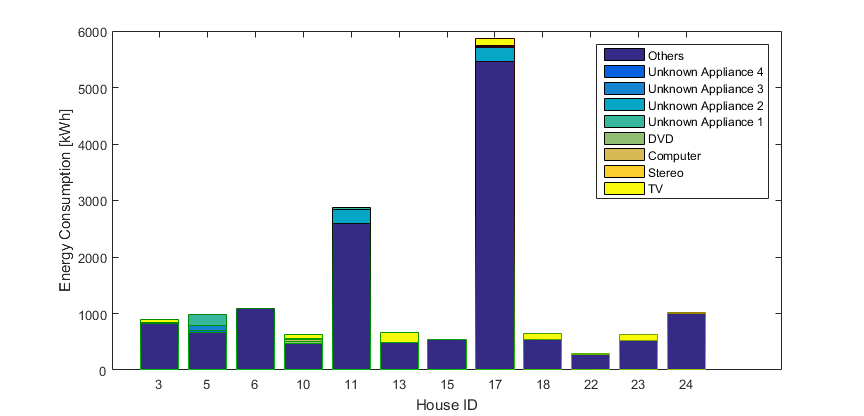
\includegraphics[width=1\textwidth]{billeder/SHGHouseUsagesV2.png}
\caption{Usage of SmartHG houses}
\label{fig:USAGEofSHG}
\end{figure}

On figure \ref{fig:USAGEofSHG} is the total consumption of the houses shown, and split up in the the different sub-meters, and a "other" category. The "other" category is the energy the main meter has used besides the energy accounted for by the sub-meters. On the figure is only shown the houses which main meter had observed a energy equal or greater than the sum of all the sub meters. This is not the case for houses that have malfunctioning main meters for a longer period of time, or for houses that have generated a lot of energy form solar cells. 

As seen on figure \ref{fig:USAGEofSHG} is the appliances equipped with sub-meters only responsible for a minor part of the total house consumption. Only the TV's and some of the unknown devices, have a relative high energy usage. The unknown devices is devices that have a sub-meter, but the appliance on the sub-meter is unknown.  

\section{Chapter Discussion}
When working and gathering big amounts of data it is important to be able to gesture about the data prior to analysing it. To look at different quality measurements researchers are able to get a good general overview of the data, and find better areas to focus on. 

It is shown that the quality also can indicate problem in the data gathering phase of a project. problems such as malfunctioning equipment, network failure or server problems can be detected by quality monitoring systems. 

For NILM applications the activity in the data, and error rate in the data can be good indications of quality. Further more is the amount of energy observed by the main meter in contrast to the energy observed by the sub-meters in a house also a good indication of the dataset quality. 
